% 若编译失败,且生成 .synctex(busy) 辅助文件,可能有两个原因:
% 1. 需要插入的图片不存在:Ctrl + F 搜索 'figure' 将这些代码注释/删除掉即可
% 2. 路径/文件名含中文或空格:更改路径/文件名即可

% --------------------- 文章宏包及相关设置 --------------------- %
% >> ------------------ 文章宏包及相关设置 ------------------ << %
% 设定文章类型与编码格式
    \documentclass[UTF8]{report}		


% 本文的特殊宏定义
\def\Im{\mathrm{\,Im\,}}
\def\Re{\mathrm{\,Re\,}}
\def\Ln{\mathrm{\,Ln\,}}
\def\Arg{\mathrm{\,Arg\,}}
\def\Arccos{\mathrm{\,Arccos\,}}
\def\Arcsin{\mathrm{\,Arcsin\,}}
\def\Arctan{\mathrm{\,Arctan\,}}

% 通用宏定义
\def\N{\mathbb{N}}
\def\F{\mathbb{F}}
\def\Z{\mathbb{Z}}
\def\Q{\mathbb{Q}}
\def\R{\mathbb{R}}
\def\C{\mathbb{C}}
\def\T{\mathbb{T}}
\def\S{\mathbb{S}}
\def\A{\mathbb{A}}
\def\I{\mathscr{I}}
\def\d{\mathrm{d}}
\def\p{\partial}


% 导入基本宏包
    \usepackage[UTF8]{ctex}     % 设置文档为中文语言
    \usepackage[colorlinks, linkcolor=blue, anchorcolor=blue, citecolor=blue, urlcolor=blue]{hyperref}  % 宏包:自动生成超链接 (此宏包与标题中的数学环境冲突)
    % \usepackage{docmute}    % 宏包:子文件导入时自动去除导言区,用于主/子文件的写作方式,\include{./51单片机笔记}即可。注:启用此宏包会导致.tex文件capacity受限。
    \usepackage{amsmath}    % 宏包:数学公式
    \usepackage{mathrsfs}   % 宏包:提供更多数学符号
    \usepackage{amssymb}    % 宏包:提供更多数学符号
    \usepackage{pifont}     % 宏包:提供了特殊符号和字体
    \usepackage{extarrows}  % 宏包:更多箭头符号
    \usepackage{multicol}   % 宏包:支持多栏 


% 文章页面margin设置
    \usepackage[a4paper, landscape]{geometry}   % 宏包:设置页面大小为A4纸,且页面为横向排版 (landscape)
        \geometry{top=0.1in}  % 1 inch= 2.46 cm, 0.75 inch = 1.85 cm
        \geometry{bottom=0.1in}
        \geometry{left=0.1in}
        \geometry{right=0.1in}   % 设置上下左右页边距
        \geometry{marginparwidth=0.2cm}    % 设置边注距离(注释、标记等)

% 配置数学环境
    \usepackage{amsthm} % 宏包:数学环境配置
    % theorem-line 环境自定义
        \newtheoremstyle{MyLineTheoremStyle}% <name>
            {11pt}% <space above>
            {11pt}% <space below>
            {}% <body font> 使用默认正文字体
            {}% <indent amount>
            {\bfseries}% <theorem head font> 设置标题项为加粗
            {:}% <punctuation after theorem head>
            {.5em}% <space after theorem head>
            {\textbf{#1}\thmnumber{#2}\ \ (\,\textbf{#3}\,)}% 设置标题内容顺序
        \theoremstyle{MyLineTheoremStyle} % 应用自定义的定理样式
        \newtheorem{LineTheorem}{Theorem.\,}
    % theorem-block 环境自定义
        \newtheoremstyle{MyBlockTheoremStyle}% <name>
            {11pt}% <space above>
            {11pt}% <space below>
            {}% <body font> 使用默认正文字体
            {}% <indent amount>
            {\bfseries}% <theorem head font> 设置标题项为加粗
            {:\\ \indent}% <punctuation after theorem head>
            {.5em}% <space after theorem head>
            {\textbf{#1}\thmnumber{#2}\ \ (\,\textbf{#3}\,)}% 设置标题内容顺序
        \theoremstyle{MyBlockTheoremStyle} % 应用自定义的定理样式
        \newtheorem{BlockTheorem}[LineTheorem]{Theorem.\,} % 使用 LineTheorem 的计数器
    % definition 环境自定义
        \newtheoremstyle{MySubsubsectionStyle}% <name>
            {11pt}% <space above>
            {11pt}% <space below>
            {}% <body font> 使用默认正文字体
            {}% <indent amount>
            {\bfseries}% <theorem head font> 设置标题项为加粗
            {:\\ \indent}% <punctuation after theorem head>
            {0pt}% <space after theorem head>
            {\textbf{#3}}% 设置标题内容顺序
        \theoremstyle{MySubsubsectionStyle} % 应用自定义的定理样式
        \newtheorem{definition}{}

%宏包:有色文本框(proof环境)及其设置
    \usepackage[dvipsnames,svgnames]{xcolor}    %设置插入的文本框颜色
    \usepackage[strict]{changepage}     % 提供一个 adjustwidth 环境
    \usepackage{framed}     % 实现方框效果
        \definecolor{graybox_color}{rgb}{0.95,0.95,0.96} % 文本框颜色。修改此行中的 rgb 数值即可改变方框纹颜色,具体颜色的rgb数值可以在网站https://colordrop.io/ 中获得。(截止目前的尝试还没有成功过,感觉单位不一样)(找到喜欢的颜色,点击下方的小眼睛,找到rgb值,复制修改即可)
        \newenvironment{graybox}{%
        \def\FrameCommand{%
        \hspace{1pt}%
        {\color{gray}\small \vrule width 2pt}%
        {\color{graybox_color}\vrule width 4pt}%
        \colorbox{graybox_color}%
        }%
        \MakeFramed{\advance\hsize-\width\FrameRestore}%
        \noindent\hspace{-4.55pt}% disable indenting first paragraph
        \begin{adjustwidth}{}{7pt}%
        \vspace{2pt}\vspace{2pt}%
        }
        {%
        \vspace{2pt}\end{adjustwidth}\endMakeFramed%
        }

% 外源代码插入设置
    % matlab 代码插入设置
    \usepackage{matlab-prettifier}
        \lstset{
            style=Matlab-editor,  % 继承matlab代码颜色等
        }
    \usepackage[most]{tcolorbox} % 引入tcolorbox包 
    \usepackage{listings} % 引入listings包
        \tcbuselibrary{listings, skins, breakable}
        \newfontfamily\codefont{Consolas} % 定义需要的 codefont 字体
        \lstdefinestyle{matlabstyle}{
            language=Matlab,
            basicstyle=\small\ttfamily\codefont,    % ttfamily 确保等宽 
            breakatwhitespace=false,
            breaklines=true,
            captionpos=b,
            keepspaces=true,
            numbers=left,
            numbersep=15pt,
            showspaces=false,
            showstringspaces=false,
            showtabs=false,
            tabsize=2
        }
        \newtcblisting{matlablisting}{
            arc=2pt,        % 圆角半径
            top=-5pt,
            bottom=-5pt,
            left=1mm,
            listing only,
            listing style=matlabstyle,
            breakable,
            colback=white   % 选一个合适的颜色
        }
% table 支持
    \usepackage{booktabs}   % 宏包:三线表
    \usepackage{tabularray} % 宏包:表格排版
    \usepackage{longtable}  % 宏包:长表格

% figure 设置
    \usepackage{graphicx}  % 支持 jpg, png, eps, pdf 图片 
    \usepackage{svg}       % 支持 svg 图片
        \svgsetup{
            % 指向 inkscape.exe 的路径
            %inkscapeexe = D:/aa_my_apps_main/Inkscape/bin/inkscape.exe, 
            inkscapeexe = D:/aa_MyApps/inkscape/bin/inkscape.exe, 
            % 一定程度上修复导入后图片文字溢出几何图形的问题
            inkscapelatex = false                 
        }
    \usepackage{subcaption} % subfigure 子图支持

% 图表进阶设置
    \usepackage{caption}    % 图注、表注
        \captionsetup[figure]{name=图}  
        \captionsetup[table]{name=表}
        \captionsetup{labelfont=bf, font=small}
    \usepackage{float}     % 图表位置浮动设置 

% 圆圈序号自定义
    \newcommand*\circled[1]{\tikz[baseline=(char.base)]{\node[shape=circle,draw,inner sep=0.8pt, line width = 0.03em] (char) {\small \bfseries #1};}}   % TikZ solution

% 列表设置
    \usepackage{enumitem}   % 宏包:列表环境设置
        \setlist[enumerate]{itemsep=0pt, parsep=0pt, topsep=0pt, partopsep=0pt, leftmargin=3.5em} 
        \setlist[itemize]{itemsep=0pt, parsep=0pt, topsep=0pt, partopsep=0pt, leftmargin=3.5em}
        \newlist{circledenum}{enumerate}{1} % 创建一个新的枚举环境  
        \setlist[circledenum,1]{  
            label=\protect\circled{\arabic*}, % 使用 \arabic* 来获取当前枚举计数器的值,并用 \circled 包装它  
            ref=\arabic*, % 如果需要引用列表项,这将决定引用格式(这里仍然使用数字)
            itemsep=0pt, parsep=0pt, topsep=0pt, partopsep=0pt, leftmargin=3.5em
        }  

% 其它设置
    % 脚注设置
        \renewcommand\thefootnote{\ding{\numexpr171+\value{footnote}}}
    % 参考文献引用设置
        \bibliographystyle{unsrt}   % 设置参考文献引用格式为unsrt
        \newcommand{\upcite}[1]{\textsuperscript{\cite{#1}}}     % 自定义上角标式引用
    % 文章序言设置
        \newcommand{\cnabstractname}{序言}
        \newenvironment{cnabstract}{%
            \par\Large
            \noindent\mbox{}\hfill{\bfseries \cnabstractname}\hfill\mbox{}\par
            \vskip 2.5ex
            }{\par\vskip 2.5ex}

% 文章默认字体设置
\usepackage{fontspec}   % 宏包:字体设置
    \setmainfont{SimSun}    % 设置中文字体为宋体字体
    \setCJKmainfont[AutoFakeBold=3]{SimSun} % 设置加粗字体为 SimSun 族,AutoFakeBold 可以调整字体粗细
    \setmainfont{Times New Roman} % 设置英文字体为Times New Roman

% 各级标题自定义设置
\usepackage{titlesec}   
\titleformat{\chapter}[hang]{\normalfont\huge\bfseries\centering}{第\,\thechapter\,章}{20pt}{}
\titlespacing*{\chapter}{0pt}{-20pt}{20pt} % 控制上方空白的大小
% section标题自定义设置 
\titleformat{\section}[hang]{\normalfont\Large\bfseries}{§\,\thesection\,}{8pt}{}
% subsubsection标题自定义设置
%\titleformat{\subsubsection}[hang]{\normalfont\bfseries}{}{8pt}{}

% --------------------- 文章宏包及相关设置 --------------------- %
% >> ------------------ 文章宏包及相关设置 ------------------ << %

% ------------------------ 文章信息区 ------------------------ %
% ------------------------ 文章信息区 ------------------------ %
% 页眉页脚设置
    \usepackage{fancyhdr}   %宏包:页眉页脚设置
        \pagestyle{fancy}
        \fancyhf{}
        \cfoot{\thepage}
        \renewcommand\headrulewidth{1pt}
        \renewcommand\footrulewidth{0pt}
        \lhead{2025.1} 
        \chead{Cheat Sheet of Principles of Electornic Circuits}    
        \rhead{dingyi233@mails.ucas.ac.cn}
%文档信息设置
    \title{这里是标题\\The Title of the Report}
    \author{丁毅\\ \footnotesize 中国科学院大学,北京 100049\\ Yi Ding \\ \footnotesize University of Chinese Academy of Sciences, Beijing 100049, China}
    \date{\footnotesize 2025.1}
% ------------------------ 文章信息区 ------------------------ %
% ------------------------ 文章信息区 ------------------------ %

% 开始编辑文章

\begin{document}
\begin{multicols*}{3}     % 多栏排版, * 号表示排满才换列
    %\setlength{\columnsep}{1cm}  % 设置栏间距 (好像无效)
\zihao{7}                % 设置全文字号大小, -4 为小四, 5 为五号

% ------------------------ 封面序言与目录 ------------------------ %
% >> --------------------- 封面序言与目录 --------------------- << %
% 封面
    % \maketitle\newpage  
    % \pagenumbering{Roman} % 页码为大写罗马数字
    % \thispagestyle{fancy}   % 显示页码、页眉等

% 序言
    %\begin{cnabstract}\zihao{6} % 设置序言字号
    %    本文为笔者本科时的某课程笔记(Notes of Linear Algebra 2, 2024.9-2025.1)。用灰色字体或灰色方框等表示对主干内容的补充、对晦涩概念的理解、定理的具体证明过程等,采用红色字体对重点部分进行强调,同时适当配有插图。这样的颜色和结构安排既突出了知识的主要框架,也保持了笔记的深度和广度,并且不会因为颜色过多而导致难以锁定文本内容,乃是尝试了多种安排后挑选出的最佳方案。如果读者有更佳的颜色和排版方案,可以将建议发送到笔者邮箱 dingyi233@mails.ucas.ac.cn,在此感谢。\par
    %    由于个人学识浅陋,认识有限,书中难免有不妥甚至错误之处,望读者不吝指正,在此感谢。

    %    本文为笔者本科时的“电路原理”课程作业(Homework of Circuit Theory, 2024.9-2025.1)。由于个人学识浅陋,认识有限,文中难免有不妥甚至错误之处,望读者不吝指正,在此感谢。我的邮箱是 dingyi233@mails.ucas.ac.cn。\par
    %\end{cnabstract}
    %\addcontentsline{toc}{chapter}{序言} % 手动添加为目录

% 目录
    %\setcounter{tocdepth}{2}                % 目录深度(为1时显示到section)
    %\tableofcontents                        % 目录页
    %\addcontentsline{toc}{chapter}{目录}    % 手动添加此页为目录
    %\thispagestyle{fancy}                   % 显示页码、页眉等 

% 收尾工作
    %\newpage    
    %\pagenumbering{arabic} 


% >> --------------------- 封面序言与目录 --------------------- << %
% ------------------------ 封面序言与目录 ------------------------ %


\chapter{基础知识}\thispagestyle{fancy} 
\section{第一章第一节}


\begin{definition}[向后加权隐式格式]

将向前差分与向后差分加权组合起来,得到:

\begin{equation}\label{公式5}
    \frac{u_{j}^{k}-u_{j}^{k-1}}{h_t}=a\theta\frac{u_{j+1}^{k}-2u_{j}^{k}+u_{j-1}^{k}}{h_x^2}+a(1-\theta)\frac{u_{j+1}^{k-1}-2u_{j}^{k-1}+u_{j-1}^{k-1}}{h_x^2}
\end{equation}

其中 $\theta \in [0, 1]$ 为权重,其截断误差 $R = a\left(\frac{1}{2}-\theta\right)h_t\left[\frac{\partial^{3}u}{\partial x^{2}\partial t}\right]_{j}^{k}+O(h_t^{2}+h_x^2)$,因此当 $\theta = \frac{1}{2}$ 时,方程具有 $O(h_t^{2}+h_x^2)$ 精度,称为 Crank-Nicolson 格式(CN 格式)。


公式 \ref{公式5} 的增长因子及稳定性条件为:

\begin{equation}
    G(h_t,\sigma)=\frac{1-4(1-\theta)ar\sin^2\frac{\sigma h}2}{1+4\theta ar\sin^2\frac{\sigma h}2}, \ \ 
    \begin{cases}
        r\leqslant\frac{1}{2a(1-2\theta)}, & \theta \in [0, \frac{1}{2}) \\ 
        \text{无条件稳定}, & \theta \in [\frac{1}{2}, 1] \\ 
    \end{cases}
\end{equation}


\begin{LineTheorem}[这是一个 Line Theorem]\label{这是一个 Line Theorem}
    你好你好你好
\end{LineTheorem}

\begin{BlockTheorem}[这是一个 Block Theorem]\label{这是一个 Block Theorem}
    你好你好你好
\end{BlockTheorem}



\begin{graybox}
\textbf{定理 \ref{这是一个 Block Theorem} 的证明:}\\
你好你好你好
\end{graybox}


\end{definition}

表格:

\begin{table}[H]
    \centering
    \caption{\textbf{符号含义与约定}}
    \label{tab:waterpump}
    \begin{tabular}{ccccc}
    \toprule
    符号 & 符号含义& 单位\\
    \midrule
    符号1& 含义1& 单位1\\
    符号2& 含义2& 单位2\\
    符号3& 含义3& 单位3\\
    符号4& 含义4& 单位4\\
    \bottomrule
    \end{tabular}
\end{table}

\subsection{线性运算器(自设计)}
图 \ref{自设计线性运算器} 是在加法器、减法器的基础上,自己设计的线性运算器,它可以实现任意数量的输入(电压)信号的任意线性运算。事实上,在此线性运算器中,电阻 $R_M$ 和电阻 $R_P$ 是关键,因为在正相信号间的比例、反相信号间的比例分别确定时,这两个电阻实现了正信号和负信号之间的比例调整,使得最终输出的正、负信号可以任意大或任意小(最小即为 0,不占任何比例)。

图中,红色端是加法信号,蓝色端是减法信号,绿色端为公共地(可只保留一个)。

\begin{figure}[H]\centering
\begin{subfigure}[t]{0.49\columnwidth}\centering
    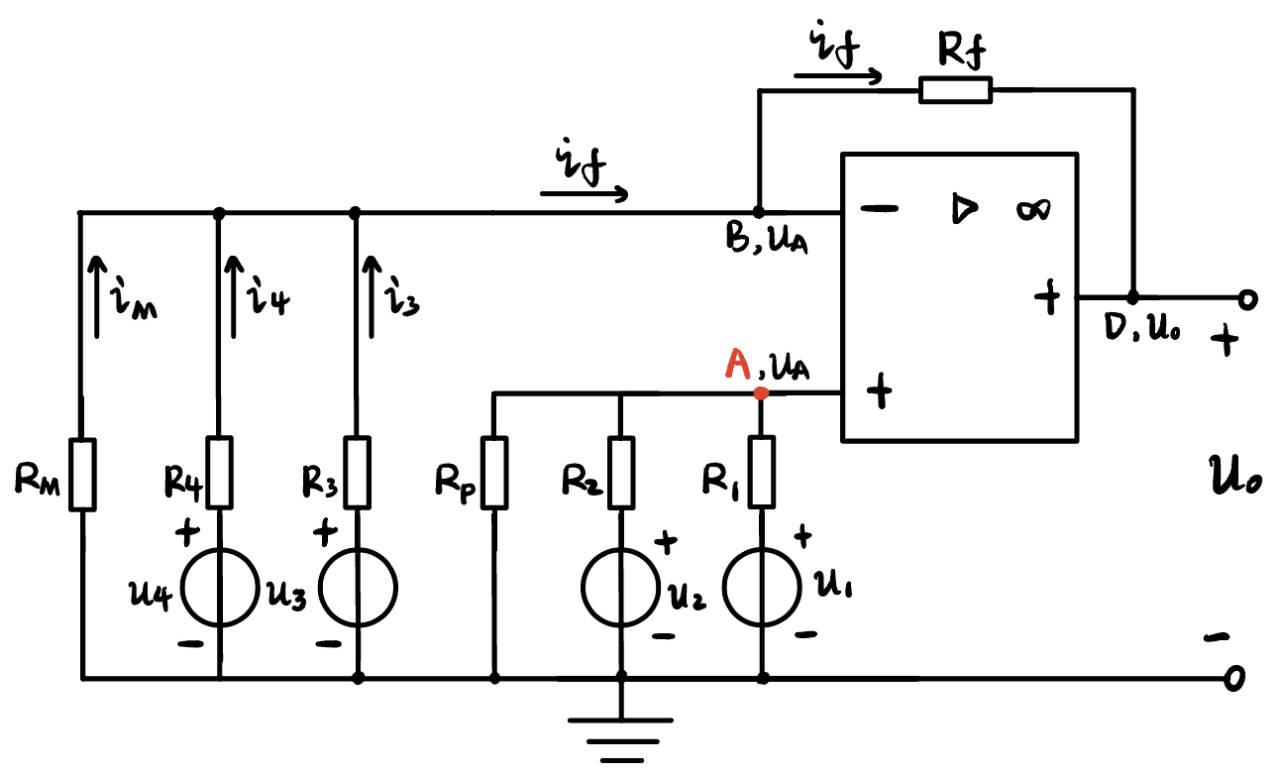
\includegraphics[height=60pt]{assets/线性运算器.png}
    \caption{\bfseries 线性运算器电路图 }
\end{subfigure}\begin{subfigure}[t]{0.49\columnwidth}\centering
    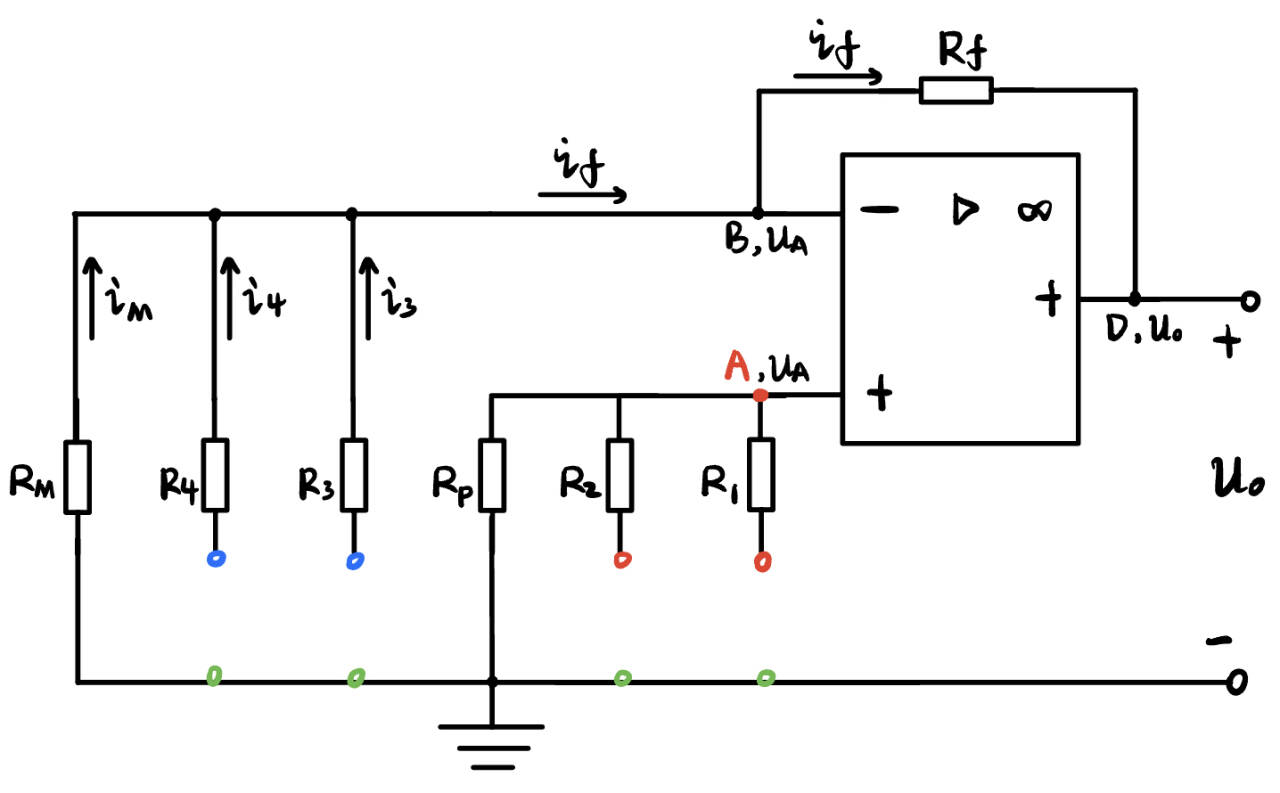
\includegraphics[height=60pt]{assets/线性运算器接线端.png}
    \caption{\bfseries 接线端示意图 }
\end{subfigure}
\caption{\bfseries 自设计线性运算器 }\label{自设计线性运算器}
\end{figure}


我们先研究图 \ref{自设计线性运算器} (a) 的输出特性,再讨论如果没有电阻 $R_M$ 或 $R_P$,输出电压会受到什么限制。输出电压的推导是简单的,先考虑点 A 的电势 $u_A$,求得:
\begin{equation}
u_A = \frac{\frac{u_1}{R_1} + \frac{u_2}{R_2}}{\frac{1}{R_1} + \frac{1}{R_2} + \frac{1}{R_p}}
\end{equation}

{\par\color{gray}\small
$u_A$ 的推导,除了列 KCL, KVL 硬解之外,还可以这样:先将 $R_p$ 断路,这样 $u_2, R_2, u_1, R_1$ 构成并联的两个实际电压源(自带电阻),容易求得此时点 A 的电势 $u_A$,并做数学上的形式变换:
\begin{equation}
u_A = \frac{R_2u_1 + R_1u_2}{R_1+R_2} =\frac{\frac{u_1}{R_1} + \frac{u_2}{R_2}}{\frac{1}{R_1} + \frac{1}{R_2} }
\end{equation}
于是,我们再并联一个实际电压源 P 后,由数学上直接推广,可以得到 $u_A$ 为:
\begin{equation}
    u_A = \frac{\frac{u_1}{R_1} + \frac{u_2}{R_2} + \frac{u_p}{R_p}}{\frac{1}{R_1} + \frac{1}{R_2} + \frac{1}{R_p}}
\end{equation}
再令 $u_p = 0$,即得图 \ref{自设计线性运算器} 中的原始 $u_A$。
\par}

再考虑左侧的电流组,并利用虚断:
\begin{align}
&\begin{cases}
    i_3 = \frac{1}{R_3}(u_3 - u_A) \\ 
    i_4 = \frac{1}{R_4}(u_4 - u_A) \\ 
    i_m = \frac{1}{R_m}(0 - u_A) \\ 
    i_f = i_3 + i_4 + i_m
\end{cases}
\Longrightarrow 
u_o = u_A - R_fi_f = u_A - R_f\left( i_3 + i_4 + i_m \right) \\ 
\Longrightarrow
u_o &=u_A - R_f \left[ 
\frac{u_3}{R_3} + \frac{u_4}{R_4} - u_A\left( \frac{1}{R_3} + \frac{1}{R_4} + \frac{1}{R_m} \right)
\right] \\ 
&=
\left[1 + R_f \left(\frac{1}{R_3} + \frac{1}{R_4} + \frac{1}{R_m} \right)\right] u_A - R_f \left( \frac{u_3}{R_3} + \frac{u_4}{R_4} \right) 
\end{align}
代入 $u_A$,整理得到:
\begin{equation}
\boxed{
    u_o= \frac{1 + \frac{R_f}{R_m} \left(\frac{1}{R_3} + \frac{1}{R_4}  \right)}{ \frac{1}{R_p} + \left(\frac{1}{R_1} + \frac{1}{R_2} \right)}\cdot \left( \frac{{\color{red} u_1}}{R_1} + \frac{{\color{red} u_2}}{R_2} \right) - R_f \cdot \left( \frac{{\color{red} u_3}}{R_3} + \frac{{\color{red} u_4}}{R_4} \right)
}
\end{equation}
这样,对于所有加法信号,可以通过 $R_1, R_2$ 间的比例来调整它们在加法中的输出比例,类似地,减法信号通过 $R_3, R_4$ 间的比例来调整它们在减法中的输出比例。最后通过 $R_f, R_m, R_p$ 来调整加法、减法之间的输出比例。在 $R_f, R_m, R_p$ 都可变时,易证(减法占比) $R_f \in [0,\ \infty)$,(加法占比)$\frac{1 + R_f \left(\frac{1}{R_3} + \frac{1}{R_4} + \frac{1}{R_m} \right)}{\frac{1}{R_1} + \frac{1}{R_2} + \frac{1}{R_p}} \in [0,\ \infty)$,于是全部系数都具有任意性,此线性运算器能够实现任意的线性运算。

上面的电路容易推广到任意输入信号个数的情形。假设有 $m$ 个加法信号 $u_{s_1}, \dots, u_{s_m}$,它们对应的串联电阻分别 $R_{s_1}, \dots, R_{s_m}$;以及$n$ 个减法信号 $u_{r_1}, \dots, u_{r_n}$,它们对应的串联阻值分别 $R_{r_1}, \dots, R_{r_n}$。直接由数学上推广出去,得到输出电压 
$u_o$ 的表达式为:

\begin{equation}
\boxed{
u_o = 
\left(
    \frac{1 + \frac{R_f}{R_m} + \displaystyle R_f\sum_{i=s_1}^{i=s_m} \frac{1}{R_i}
    }{
        \frac{1}{R_p} + \displaystyle \sum_{i=r_1}^{i=r_n} \frac{1}{R_i}
    }
\right)\cdot \displaystyle\sum_{i=s_1}^{i=s_m} \frac{{\color{red} u_i}}{R_i}  - R_f \cdot  \displaystyle\sum_{i=r_1}^{i=r_n} \frac{{\color{red} u_i}}{R_i}
}
\end{equation}

此线性运算器的具体仿真示例见 Homework 3.

% ------------------------- 参考文献 ------------------------- %
% >> ---------------------- 参考文献 ---------------------- << %
%\nocite{*}
%\bibliography{re}
%\thispagestyle{fancy} 
%\addcontentsline{toc}{chapter}{参考文献}
% ------------------------- 参考文献 ------------------------- %
% >> ---------------------- 参考文献 ---------------------- << %


% --------------------------- 附录 --------------------------- %
% >> ------------------------ 附录 ------------------------ << %

%% 附录设置
%\newpage
%\appendix
%% chapter 标题自定义设置
%\titleformat{\chapter}[hang]{\normalfont\huge\bfseries\centering}{}{20pt}{}
%\titlespacing*{\chapter}{0pt}{-25pt}{8pt} % 控制上方空白的大小
%% section 标题自定义设置 
%\titleformat{\section}[hang]{\normalfont\centering\Large\bfseries}%{\thesection}{8pt}{}
%
%% 附录 A
%\chapter*{附录 A. 中英文对照表}\addcontentsline{toc}{chapter}{附录 A. 中英文对照%表}   
%\thispagestyle{fancy} 
%\setcounter{section}{0}   
%\renewcommand\thesection{A.\arabic{section}}   
%\renewcommand{\thefigure}{A.\arabic{figure}} 
%\renewcommand{\thetable}{A.\arabic{table}}
%
%\section{中英文对照表}
%\begin{multicols}{2}  
%
%    \begin{table}[H]\centering
%    \caption{\textbf{中英文对照表}}
%    \begin{tabular}{cccccccc}\toprule
%        English & 中文 \\
%        \midrule
%        voltage            & 电压 \\
%        current            & 电流 \\
%        power              & 功率 \\
%        resistance         & 电阻 \\
%        conductance        & 电导 \\
%        inductance         & 电感 \\
%        capacitance        & 电容 \\
%        frequency          & 频率 \\
%        circuit            & 电路 \\
%        circuit element    & 电流元件 \\
%        signal             & 信号 \\
%        circuit analysis   & 电路分析 \\
%        circuit synthesis  & 电路综合 \\
%        circuit design     & 电路设计 \\
%        circuit topology   & 电路拓扑 \\
%        \bottomrule
%    \end{tabular}
%    \end{table}
%    
%    \begin{table}[H]\centering
%        \caption{\textbf{中英文对照表}}
%        \begin{tabular}{cccccccc}\toprule
%            English & 中文 \\
%            \midrule
%            voltage            & 电压 \\
%            current            & 电流 \\
%            power              & 功率 \\
%            resistance         & 电阻 \\
%            conductance        & 电导 \\
%            inductance         & 电感 \\
%            capacitance        & 电容 \\
%            frequency          & 频率 \\
%            circuit            & 电路 \\
%            circuit element    & 电流元件 \\
%            signal             & 信号 \\
%            circuit analysis   & 电路分析 \\
%            circuit synthesis  & 电路综合 \\
%            circuit design     & 电路设计 \\
%            circuit topology   & 电路拓扑 \\
%            \bottomrule
%        \end{tabular}
%    \end{table}
%\end{multicols} 
%    
%\section{支撑材料列表} 
%
%\begin{center}
%  这里插入一张图片(类似思维导图那种)
%\end{center}
%
%
%% 附录 B
%\chapter*{附录 B. Matlab 代码}\addcontentsline{toc}{chapter}{附录 B. Matlab 代%码}   
%\thispagestyle{fancy} 
%\setcounter{section}{0}   
%\renewcommand\thesection{B.\arabic{section}}   
%\renewcommand{\thefigure}{B.\arabic{figure}} 
%\renewcommand{\thetable}{B.\arabic{table}}
%
%% 注意:listing环境中手动输入的代码需要顶格写
%
%\begin{matlablisting}
%% MATLAB code here
%x = 0:0.1:2*pi;
%y = sin(x);
%plot(x, y);
%xlabel('x');
%ylabel('sin(x)');
%title('Sine Function');
%% ... (MATLAB code here,最好是插入文件)
%% MATLAB code here
%x = 0:0.1:2*pi;
%y = sin(x);
%plot(x, y);
%xlabel('x');
%ylabel('sin(x)');
%title('Sine Function');
%% ... (MATLAB code here,最好是插入文件)
%% MATLAB code here
%x = 0:0.1:2*pi;
%y = sin(x);
%plot(x, y);
%xlabel('x');
%ylabel('sin(x)');
%title('Sine Function');
%% ... (MATLAB code here,最好是插入文件)
%% MATLAB code here
%x = 0:0.1:2*pi;
%y = sin(x);
%plot(x, y);
%xlabel('x');
%ylabel('sin(x)');
%title('Sine Function');
%% ... (MATLAB code here,最好是插入文件)
%% MATLAB code here
%x = 0:0.1:2*pi;
%y = sin(x);
%plot(x, y);
%xlabel('x');
%ylabel('sin(x)');
%title('Sine Function');
%% ... (MATLAB code here,最好是插入文件)
%% MATLAB code here
%x = 0:0.1:2*pi;
%y = sin(x);
%plot(x, y);
%xlabel('x');
%ylabel('sin(x)');
%title('Sine Function');
%% ... (MATLAB code here,最好是插入文件)% ... (MATLAB code here,最好是插入文件)%% ... (MATLAB code here,最好是插入文件)% ... (MATLAB code here,最好是插入文件)%% ... (MATLAB code here,最好是插入文件)A
%% MATLAB code here
%x = 0:0.1:2*pi;
%y = sin(x);
%plot(x, y);
%xlabel('x');
%ylabel('sin(x)');
%title('Sine Function');
%% ... (MATLAB code here,最好是插入文件)
%\end{matlablisting}

% --------------------------- 附录 --------------------------- %
% >> ------------------------ 附录 ------------------------ << %
\end{multicols*}
\end{document}



% VScode 常用快捷键:

% F2:                       变量重命名
% Ctrl + Enter:             行中换行
% Alt + up/down:            上下移行
% 鼠标中键 + 移动:           快速多光标
% Shift + Alt + up/down:    上下复制
% Ctrl + left/right:        左右跳单词
% Ctrl + Backspace/Delete:  左右删单词    
% Shift + Delete:           删除此行
% Ctrl + J:                 打开 VScode 下栏(输出栏)
% Ctrl + B:                 打开 VScode 左栏(目录栏)
% Ctrl + `:                 打开 VScode 终端栏
% Ctrl + 0:                 定位文件
% Ctrl + Tab:               切换已打开的文件(切标签)
% Ctrl + Shift + P:         打开全局命令(设置)

% Latex 常用快捷键

% Ctrl + Alt + J:           由代码定位到PDF
% 


% Git提交规范:
% update: Linear Algebra 2 notes
% add: Linear Algebra 2 notes
% import: Linear Algebra 2 notes
% delete: Linear Algebra 2 notes

